circle (  1.4);% Created by tikzDevice version 0.9 on 2016-01-08 20:52:20
% !TEX encoding = UTF-8 Unicode
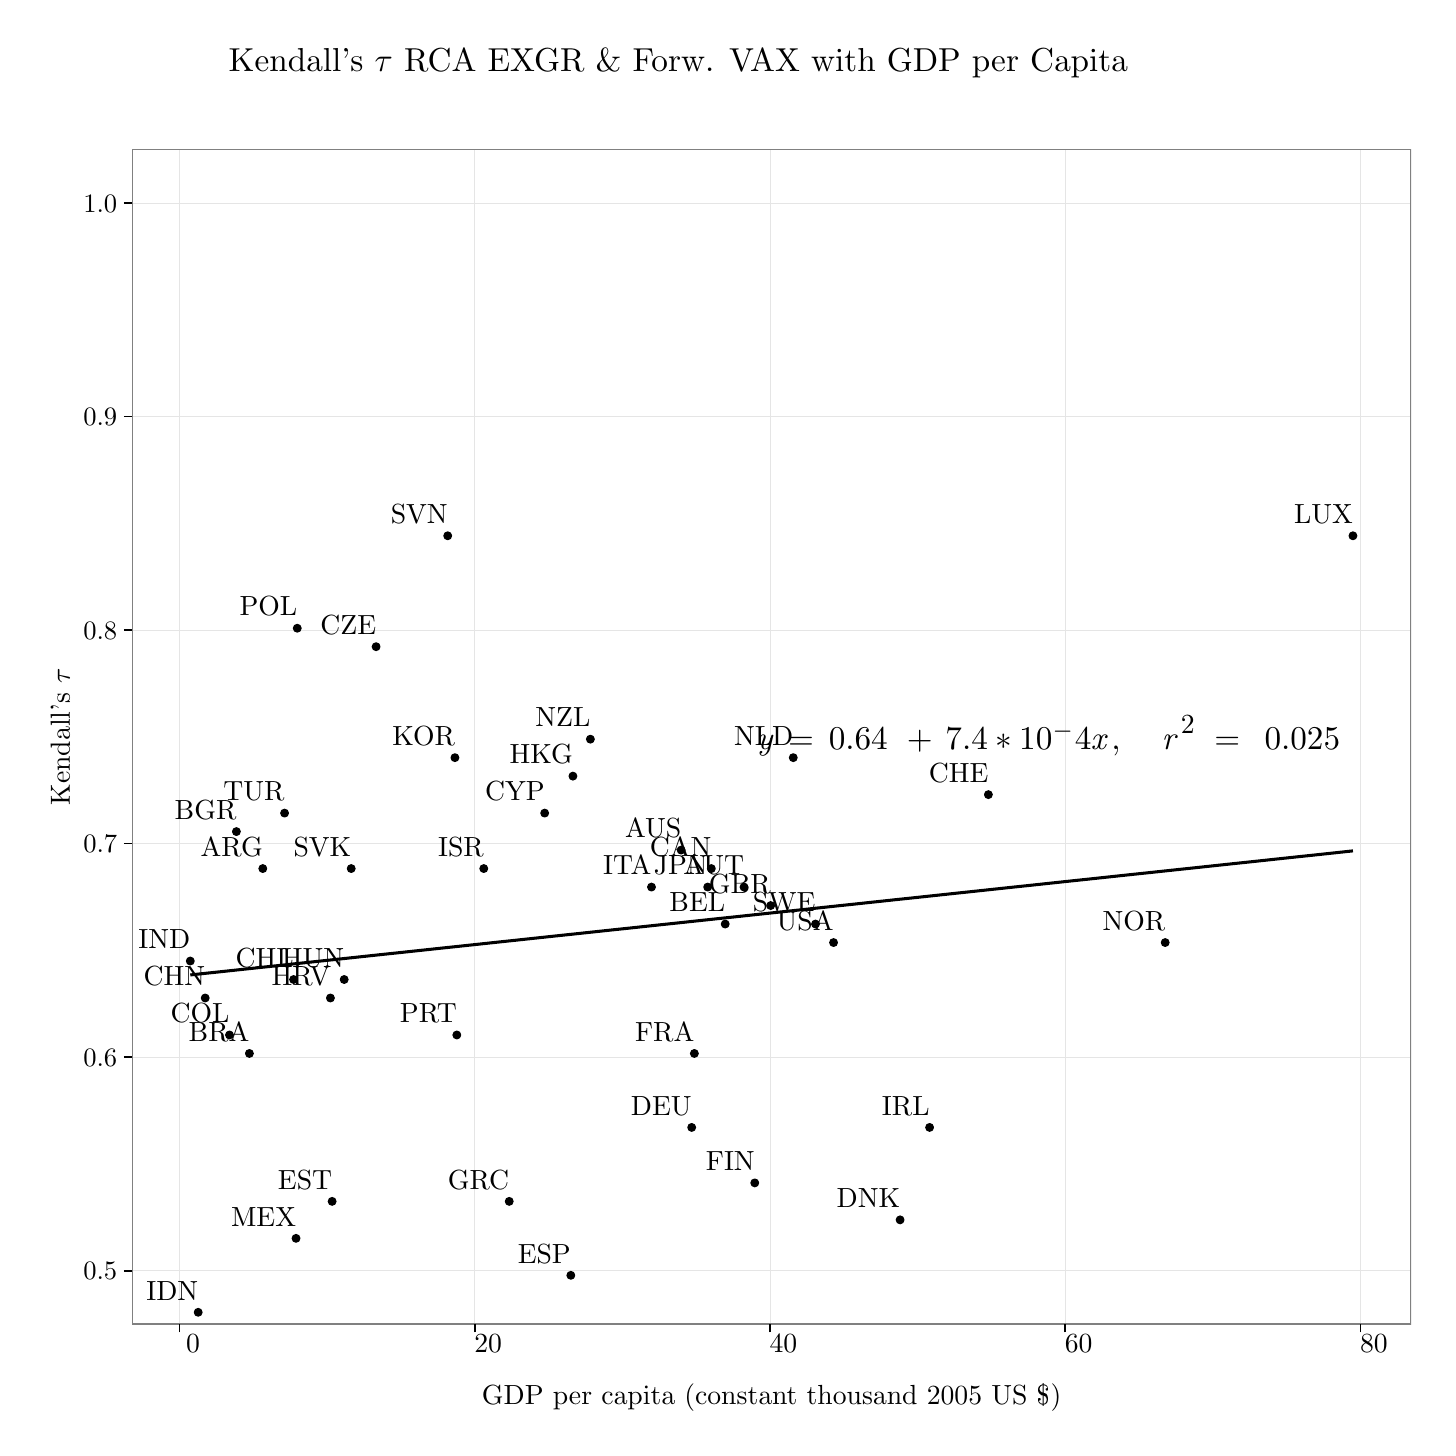
\begin{tikzpicture}[x=1pt,y=1pt]
\definecolor{fillColor}{RGB}{255,255,255}
\path[use as bounding box,fill=fillColor,fill opacity=0.00] (0,0) rectangle (505.89,505.89);
\begin{scope}
\path[clip] (  0.00,  0.00) rectangle (505.89,505.89);
\definecolor{drawColor}{RGB}{255,255,255}
\definecolor{fillColor}{RGB}{255,255,255}

\path[draw=drawColor,line width= 0.6pt,line join=round,line cap=round,fill=fillColor] (  0.00, -0.00) rectangle (505.89,505.89);
\end{scope}
\begin{scope}
\path[clip] ( 37.75, 37.43) rectangle (499.89,461.83);
\definecolor{fillColor}{RGB}{255,255,255}

\path[fill=fillColor] ( 37.75, 37.43) rectangle (499.89,461.83);
\definecolor{drawColor}{gray}{0.90}

\path[draw=drawColor,line width= 0.2pt,line join=round] ( 37.75, 56.72) --
	(499.89, 56.72);

\path[draw=drawColor,line width= 0.2pt,line join=round] ( 37.75,133.88) --
	(499.89,133.88);

\path[draw=drawColor,line width= 0.2pt,line join=round] ( 37.75,211.05) --
	(499.89,211.05);

\path[draw=drawColor,line width= 0.2pt,line join=round] ( 37.75,288.21) --
	(499.89,288.21);

\path[draw=drawColor,line width= 0.2pt,line join=round] ( 37.75,365.38) --
	(499.89,365.38);

\path[draw=drawColor,line width= 0.2pt,line join=round] ( 37.75,442.54) --
	(499.89,442.54);

\path[draw=drawColor,line width= 0.2pt,line join=round] ( 54.87, 37.43) --
	( 54.87,461.83);

\path[draw=drawColor,line width= 0.2pt,line join=round] (161.55, 37.43) --
	(161.55,461.83);

\path[draw=drawColor,line width= 0.2pt,line join=round] (268.23, 37.43) --
	(268.23,461.83);

\path[draw=drawColor,line width= 0.2pt,line join=round] (374.90, 37.43) --
	(374.90,461.83);

\path[draw=drawColor,line width= 0.2pt,line join=round] (481.58, 37.43) --
	(481.58,461.83);
\definecolor{drawColor}{RGB}{0,0,0}
\definecolor{fillColor}{RGB}{0,0,0}

\path[draw=drawColor,line width= 0.4pt,line join=round,line cap=round,fill=fillColor] ( 84.96,202.03) circle (  1.4);

\path[draw=drawColor,line width= 0.4pt,line join=round,line cap=round,fill=fillColor] (236.13,208.71) circle (  1.4);

\path[draw=drawColor,line width= 0.4pt,line join=round,line cap=round,fill=fillColor] (258.85,195.35) circle (  1.4);

\path[draw=drawColor,line width= 0.4pt,line join=round,line cap=round,fill=fillColor] (252.05,181.99) circle (  1.4);

\path[draw=drawColor,line width= 0.4pt,line join=round,line cap=round,fill=fillColor] ( 75.42,215.39) circle (  1.4);

\path[draw=drawColor,line width= 0.4pt,line join=round,line cap=round,fill=fillColor] ( 80.12,135.22) circle (  1.4);

\path[draw=drawColor,line width= 0.4pt,line join=round,line cap=round,fill=fillColor] (247.04,202.03) circle (  1.4);

\path[draw=drawColor,line width= 0.4pt,line join=round,line cap=round,fill=fillColor] (347.15,228.75) circle (  1.4);

\path[draw=drawColor,line width= 0.4pt,line join=round,line cap=round,fill=fillColor] ( 96.09,161.94) circle (  1.4);

\path[draw=drawColor,line width= 0.4pt,line join=round,line cap=round,fill=fillColor] ( 64.15,155.26) circle (  1.4);

\path[draw=drawColor,line width= 0.4pt,line join=round,line cap=round,fill=fillColor] ( 72.93,141.90) circle (  1.4);

\path[draw=drawColor,line width= 0.4pt,line join=round,line cap=round,fill=fillColor] (186.82,222.07) circle (  1.4);

\path[draw=drawColor,line width= 0.4pt,line join=round,line cap=round,fill=fillColor] (125.90,282.20) circle (  1.4);

\path[draw=drawColor,line width= 0.4pt,line join=round,line cap=round,fill=fillColor] (239.94,108.49) circle (  1.4);

\path[draw=drawColor,line width= 0.4pt,line join=round,line cap=round,fill=fillColor] (315.25, 75.09) circle (  1.4);

\path[draw=drawColor,line width= 0.4pt,line join=round,line cap=round,fill=fillColor] (196.27, 55.05) circle (  1.4);

\path[draw=drawColor,line width= 0.4pt,line join=round,line cap=round,fill=fillColor] (110.01, 81.77) circle (  1.4);

\path[draw=drawColor,line width= 0.4pt,line join=round,line cap=round,fill=fillColor] (262.73, 88.45) circle (  1.4);

\path[draw=drawColor,line width= 0.4pt,line join=round,line cap=round,fill=fillColor] (240.91,135.22) circle (  1.4);

\path[draw=drawColor,line width= 0.4pt,line join=round,line cap=round,fill=fillColor] (268.48,188.67) circle (  1.4);

\path[draw=drawColor,line width= 0.4pt,line join=round,line cap=round,fill=fillColor] (174.01, 81.77) circle (  1.4);

\path[draw=drawColor,line width= 0.4pt,line join=round,line cap=round,fill=fillColor] (197.02,235.43) circle (  1.4);

\path[draw=drawColor,line width= 0.4pt,line join=round,line cap=round,fill=fillColor] (109.40,155.26) circle (  1.4);

\path[draw=drawColor,line width= 0.4pt,line join=round,line cap=round,fill=fillColor] (114.37,161.94) circle (  1.4);

\path[draw=drawColor,line width= 0.4pt,line join=round,line cap=round,fill=fillColor] ( 61.61, 41.69) circle (  1.4);

\path[draw=drawColor,line width= 0.4pt,line join=round,line cap=round,fill=fillColor] ( 58.76,168.62) circle (  1.4);

\path[draw=drawColor,line width= 0.4pt,line join=round,line cap=round,fill=fillColor] (325.91,108.49) circle (  1.4);

\path[draw=drawColor,line width= 0.4pt,line join=round,line cap=round,fill=fillColor] (164.81,202.03) circle (  1.4);

\path[draw=drawColor,line width= 0.4pt,line join=round,line cap=round,fill=fillColor] (225.41,195.35) circle (  1.4);

\path[draw=drawColor,line width= 0.4pt,line join=round,line cap=round,fill=fillColor] (245.72,195.35) circle (  1.4);

\path[draw=drawColor,line width= 0.4pt,line join=round,line cap=round,fill=fillColor] (154.39,242.11) circle (  1.4);

\path[draw=drawColor,line width= 0.4pt,line join=round,line cap=round,fill=fillColor] (478.88,322.28) circle (  1.4);

\path[draw=drawColor,line width= 0.4pt,line join=round,line cap=round,fill=fillColor] ( 96.97, 68.41) circle (  1.4);

\path[draw=drawColor,line width= 0.4pt,line join=round,line cap=round,fill=fillColor] (276.64,242.11) circle (  1.4);

\path[draw=drawColor,line width= 0.4pt,line join=round,line cap=round,fill=fillColor] (411.04,175.30) circle (  1.4);

\path[draw=drawColor,line width= 0.4pt,line join=round,line cap=round,fill=fillColor] (203.33,248.79) circle (  1.4);

\path[draw=drawColor,line width= 0.4pt,line join=round,line cap=round,fill=fillColor] ( 97.41,288.88) circle (  1.4);

\path[draw=drawColor,line width= 0.4pt,line join=round,line cap=round,fill=fillColor] (155.07,141.90) circle (  1.4);

\path[draw=drawColor,line width= 0.4pt,line join=round,line cap=round,fill=fillColor] (116.91,202.03) circle (  1.4);

\path[draw=drawColor,line width= 0.4pt,line join=round,line cap=round,fill=fillColor] (151.78,322.28) circle (  1.4);

\path[draw=drawColor,line width= 0.4pt,line join=round,line cap=round,fill=fillColor] (284.68,181.99) circle (  1.4);

\path[draw=drawColor,line width= 0.4pt,line join=round,line cap=round,fill=fillColor] ( 92.83,222.07) circle (  1.4);

\path[draw=drawColor,line width= 0.4pt,line join=round,line cap=round,fill=fillColor] (291.20,175.30) circle (  1.4);

\node[text=drawColor,anchor=base east,inner sep=0pt, outer sep=0pt, scale=  1] at ( 84.96,206.47) {ARG};

\node[text=drawColor,anchor=base east,inner sep=0pt, outer sep=0pt, scale=  1] at (236.13,213.15) {AUS};

\node[text=drawColor,anchor=base east,inner sep=0pt, outer sep=0pt, scale=  1] at (258.85,199.79) {AUT};

\node[text=drawColor,anchor=base east,inner sep=0pt, outer sep=0pt, scale=  1] at (252.05,186.43) {BEL};

\node[text=drawColor,anchor=base east,inner sep=0pt, outer sep=0pt, scale=  1] at ( 75.42,219.83) {BGR};

\node[text=drawColor,anchor=base east,inner sep=0pt, outer sep=0pt, scale=  1] at ( 80.12,139.66) {BRA};

\node[text=drawColor,anchor=base east,inner sep=0pt, outer sep=0pt, scale=  1] at (247.04,206.47) {CAN};

\node[text=drawColor,anchor=base east,inner sep=0pt, outer sep=0pt, scale=  1] at (347.15,233.19) {CHE};

\node[text=drawColor,anchor=base east,inner sep=0pt, outer sep=0pt, scale=  1] at ( 96.09,166.38) {CHL};

\node[text=drawColor,anchor=base east,inner sep=0pt, outer sep=0pt, scale=  1] at ( 64.15,159.70) {CHN};

\node[text=drawColor,anchor=base east,inner sep=0pt, outer sep=0pt, scale=  1] at ( 72.93,146.34) {COL};

\node[text=drawColor,anchor=base east,inner sep=0pt, outer sep=0pt, scale=  1] at (186.82,226.51) {CYP};

\node[text=drawColor,anchor=base east,inner sep=0pt, outer sep=0pt, scale=  1] at (125.90,286.64) {CZE};

\node[text=drawColor,anchor=base east,inner sep=0pt, outer sep=0pt, scale=  1] at (239.94,112.94) {DEU};

\node[text=drawColor,anchor=base east,inner sep=0pt, outer sep=0pt, scale=  1] at (315.25, 79.53) {DNK};

\node[text=drawColor,anchor=base east,inner sep=0pt, outer sep=0pt, scale=  1] at (196.27, 59.49) {ESP};

\node[text=drawColor,anchor=base east,inner sep=0pt, outer sep=0pt, scale=  1] at (110.01, 86.21) {EST};

\node[text=drawColor,anchor=base east,inner sep=0pt, outer sep=0pt, scale=  1] at (262.73, 92.89) {FIN};

\node[text=drawColor,anchor=base east,inner sep=0pt, outer sep=0pt, scale=  1] at (240.91,139.66) {FRA};

\node[text=drawColor,anchor=base east,inner sep=0pt, outer sep=0pt, scale=  1] at (268.48,193.11) {GBR};

\node[text=drawColor,anchor=base east,inner sep=0pt, outer sep=0pt, scale=  1] at (174.01, 86.21) {GRC};

\node[text=drawColor,anchor=base east,inner sep=0pt, outer sep=0pt, scale=  1] at (197.02,239.87) {HKG};

\node[text=drawColor,anchor=base east,inner sep=0pt, outer sep=0pt, scale=  1] at (109.40,159.70) {HRV};

\node[text=drawColor,anchor=base east,inner sep=0pt, outer sep=0pt, scale=  1] at (114.37,166.38) {HUN};

\node[text=drawColor,anchor=base east,inner sep=0pt, outer sep=0pt, scale=  1] at ( 61.61, 46.13) {IDN};

\node[text=drawColor,anchor=base east,inner sep=0pt, outer sep=0pt, scale=  1] at ( 58.76,173.07) {IND};

\node[text=drawColor,anchor=base east,inner sep=0pt, outer sep=0pt, scale=  1] at (325.91,112.94) {IRL};

\node[text=drawColor,anchor=base east,inner sep=0pt, outer sep=0pt, scale=  1] at (164.81,206.47) {ISR};

\node[text=drawColor,anchor=base east,inner sep=0pt, outer sep=0pt, scale=  1] at (225.41,199.79) {ITA};

\node[text=drawColor,anchor=base east,inner sep=0pt, outer sep=0pt, scale=  1] at (245.72,199.79) {JPN};

\node[text=drawColor,anchor=base east,inner sep=0pt, outer sep=0pt, scale=  1] at (154.39,246.56) {KOR};

\node[text=drawColor,anchor=base east,inner sep=0pt, outer sep=0pt, scale=  1] at (478.88,326.73) {LUX};

\node[text=drawColor,anchor=base east,inner sep=0pt, outer sep=0pt, scale=  1] at ( 96.97, 72.85) {MEX};

\node[text=drawColor,anchor=base east,inner sep=0pt, outer sep=0pt, scale=  1] at (276.64,246.56) {NLD};

\node[text=drawColor,anchor=base east,inner sep=0pt, outer sep=0pt, scale=  1] at (411.04,179.75) {NOR};

\node[text=drawColor,anchor=base east,inner sep=0pt, outer sep=0pt, scale=  1] at (203.33,253.24) {NZL};

\node[text=drawColor,anchor=base east,inner sep=0pt, outer sep=0pt, scale=  1] at ( 97.41,293.32) {POL};

\node[text=drawColor,anchor=base east,inner sep=0pt, outer sep=0pt, scale=  1] at (155.07,146.34) {PRT};

\node[text=drawColor,anchor=base east,inner sep=0pt, outer sep=0pt, scale=  1] at (116.91,206.47) {SVK};

\node[text=drawColor,anchor=base east,inner sep=0pt, outer sep=0pt, scale=  1] at (151.78,326.73) {SVN};

\node[text=drawColor,anchor=base east,inner sep=0pt, outer sep=0pt, scale=  1] at (284.68,186.43) {SWE};

\node[text=drawColor,anchor=base east,inner sep=0pt, outer sep=0pt, scale=  1] at ( 92.83,226.51) {TUR};

\node[text=drawColor,anchor=base east,inner sep=0pt, outer sep=0pt, scale=  1] at (291.20,179.75) {USA};

\path[draw=drawColor,line width= 1.1pt,line join=round] ( 58.76,163.59) --
	( 64.08,164.16) --
	( 69.39,164.72) --
	( 74.71,165.29) --
	( 80.03,165.86) --
	( 85.35,166.43) --
	( 90.67,166.99) --
	( 95.98,167.56) --
	(101.30,168.13) --
	(106.62,168.70) --
	(111.94,169.26) --
	(117.26,169.83) --
	(122.57,170.40) --
	(127.89,170.97) --
	(133.21,171.53) --
	(138.53,172.10) --
	(143.85,172.67) --
	(149.16,173.24) --
	(154.48,173.80) --
	(159.80,174.37) --
	(165.12,174.94) --
	(170.44,175.51) --
	(175.75,176.07) --
	(181.07,176.64) --
	(186.39,177.21) --
	(191.71,177.78) --
	(197.03,178.34) --
	(202.34,178.91) --
	(207.66,179.48) --
	(212.98,180.05) --
	(218.30,180.61) --
	(223.62,181.18) --
	(228.94,181.75) --
	(234.25,182.31) --
	(239.57,182.88) --
	(244.89,183.45) --
	(250.21,184.02) --
	(255.53,184.58) --
	(260.84,185.15) --
	(266.16,185.72) --
	(271.48,186.29) --
	(276.80,186.85) --
	(282.12,187.42) --
	(287.43,187.99) --
	(292.75,188.56) --
	(298.07,189.12) --
	(303.39,189.69) --
	(308.71,190.26) --
	(314.02,190.83) --
	(319.34,191.39) --
	(324.66,191.96) --
	(329.98,192.53) --
	(335.30,193.10) --
	(340.61,193.66) --
	(345.93,194.23) --
	(351.25,194.80) --
	(356.57,195.37) --
	(361.89,195.93) --
	(367.20,196.50) --
	(372.52,197.07) --
	(377.84,197.64) --
	(383.16,198.20) --
	(388.48,198.77) --
	(393.79,199.34) --
	(399.11,199.91) --
	(404.43,200.47) --
	(409.75,201.04) --
	(415.07,201.61) --
	(420.39,202.17) --
	(425.70,202.74) --
	(431.02,203.31) --
	(436.34,203.88) --
	(441.66,204.44) --
	(446.98,205.01) --
	(452.29,205.58) --
	(457.61,206.15) --
	(462.93,206.71) --
	(468.25,207.28) --
	(473.57,207.85) --
	(478.88,208.42);

\node[text=drawColor,anchor=base west,inner sep=0pt, outer sep=0pt, scale=  1.2] at (263.34,244.91) {\itshape y};

\node[text=drawColor,anchor=base west,inner sep=0pt, outer sep=0pt, scale=  1.2] at (274.79,244.91) {=};

\node[text=drawColor,anchor=base west,inner sep=0pt, outer sep=0pt, scale=  1.2] at (289.48,244.91) {0.64};

\node[text=drawColor,anchor=base west,inner sep=0pt, outer sep=0pt, scale=  1.2] at (317.67,244.91) {+};

\node[text=drawColor,anchor=base west,inner sep=0pt, outer sep=0pt, scale=  1.2] at (331.63,244.91) {$7.4*10{^-4}$};

\node[text=drawColor,anchor=base west,inner sep=0pt, outer sep=0pt, scale=  1.2] at (384.06,244.91) {\itshape x};

\node[text=drawColor,anchor=base west,inner sep=0pt, outer sep=0pt, scale=  1.2] at (391.58,244.91) {,};

\node[text=drawColor,anchor=base west,inner sep=0pt, outer sep=0pt, scale=  1.2] at (395.53,244.91) { };

\node[text=drawColor,anchor=base west,inner sep=0pt, outer sep=0pt, scale=  1.2] at (402.64,244.91) { };

\node[text=drawColor,anchor=base west,inner sep=0pt, outer sep=0pt, scale=  1.2] at (409.76,244.91) {\itshape r};

\node[text=drawColor,anchor=base west,inner sep=0pt, outer sep=0pt, scale=  1.00] at (416.68,250.73) {2};

\node[text=drawColor,anchor=base west,inner sep=0pt, outer sep=0pt, scale=  1.2] at (421.65,244.91) { };

\node[text=drawColor,anchor=base west,inner sep=0pt, outer sep=0pt, scale=  1.2] at (428.77,244.91) {=};

\node[text=drawColor,anchor=base west,inner sep=0pt, outer sep=0pt, scale=  1.2] at (439.83,244.91) { };

\node[text=drawColor,anchor=base west,inner sep=0pt, outer sep=0pt, scale=  1.2] at (446.94,244.91) {0.025};
\definecolor{drawColor}{gray}{0.50}

\path[draw=drawColor,line width= 0.6pt,line join=round,line cap=round] ( 37.75, 37.43) rectangle (499.89,461.83);
\end{scope}
\begin{scope}
\path[clip] (  0.00,  0.00) rectangle (505.89,505.89);
\definecolor{drawColor}{RGB}{0,0,0}

\node[text=drawColor,anchor=base east,inner sep=0pt, outer sep=0pt, scale=  0.96] at ( 32.35, 53.41) {0.5};

\node[text=drawColor,anchor=base east,inner sep=0pt, outer sep=0pt, scale=  0.96] at ( 32.35,130.58) {0.6};

\node[text=drawColor,anchor=base east,inner sep=0pt, outer sep=0pt, scale=  0.96] at ( 32.35,207.74) {0.7};

\node[text=drawColor,anchor=base east,inner sep=0pt, outer sep=0pt, scale=  0.96] at ( 32.35,284.91) {0.8};

\node[text=drawColor,anchor=base east,inner sep=0pt, outer sep=0pt, scale=  0.96] at ( 32.35,362.07) {0.9};

\node[text=drawColor,anchor=base east,inner sep=0pt, outer sep=0pt, scale=  0.96] at ( 32.35,439.24) {1.0};
\end{scope}
\begin{scope}
\path[clip] (  0.00,  0.00) rectangle (505.89,505.89);
\definecolor{drawColor}{RGB}{0,0,0}

\path[draw=drawColor,line width= 0.6pt,line join=round] ( 34.75, 56.72) --
	( 37.75, 56.72);

\path[draw=drawColor,line width= 0.6pt,line join=round] ( 34.75,133.88) --
	( 37.75,133.88);

\path[draw=drawColor,line width= 0.6pt,line join=round] ( 34.75,211.05) --
	( 37.75,211.05);

\path[draw=drawColor,line width= 0.6pt,line join=round] ( 34.75,288.21) --
	( 37.75,288.21);

\path[draw=drawColor,line width= 0.6pt,line join=round] ( 34.75,365.38) --
	( 37.75,365.38);

\path[draw=drawColor,line width= 0.6pt,line join=round] ( 34.75,442.54) --
	( 37.75,442.54);
\end{scope}
\begin{scope}
\path[clip] (  0.00,  0.00) rectangle (505.89,505.89);
\definecolor{drawColor}{RGB}{0,0,0}

\path[draw=drawColor,line width= 0.6pt,line join=round] ( 54.87, 34.43) --
	( 54.87, 37.43);

\path[draw=drawColor,line width= 0.6pt,line join=round] (161.55, 34.43) --
	(161.55, 37.43);

\path[draw=drawColor,line width= 0.6pt,line join=round] (268.23, 34.43) --
	(268.23, 37.43);

\path[draw=drawColor,line width= 0.6pt,line join=round] (374.90, 34.43) --
	(374.90, 37.43);

\path[draw=drawColor,line width= 0.6pt,line join=round] (481.58, 34.43) --
	(481.58, 37.43);
\end{scope}
\begin{scope}
\path[clip] (  0.00,  0.00) rectangle (505.89,505.89);
\definecolor{drawColor}{RGB}{0,0,0}

\node[text=drawColor,rotate= 0.00,anchor=base,inner sep=0pt, outer sep=0pt, scale=  1.00] at ( 59.74, 27.16) {0};

\node[text=drawColor,rotate= 0.00,anchor=base,inner sep=0pt, outer sep=0pt, scale=  1.00] at (166.42, 27.16) {20};

\node[text=drawColor,rotate= 0.00,anchor=base,inner sep=0pt, outer sep=0pt, scale=  1.00] at (273.10, 27.16) {40};

\node[text=drawColor,rotate= 0.00,anchor=base,inner sep=0pt, outer sep=0pt, scale=  1.00] at (379.77, 27.16) {60};

\node[text=drawColor,rotate= 0.00,anchor=base,inner sep=0pt, outer sep=0pt, scale=  1.00] at (486.45, 27.16) {80};
\end{scope}
\begin{scope}
\path[clip] (  0.00,  0.00) rectangle (505.89,505.89);
\definecolor{drawColor}{RGB}{0,0,0}

\node[text=drawColor,anchor=base,inner sep=0pt, outer sep=0pt, scale=  1.00] at (268.82,  8.40) {GDP per capita (constant thousand 2005 US \$)};
\end{scope}
\begin{scope}
\path[clip] (  0.00,  0.00) rectangle (505.89,505.89);
\definecolor{drawColor}{RGB}{0,0,0}

\node[text=drawColor,rotate= 90.00,anchor=base,inner sep=0pt, outer sep=0pt, scale=  1.00] at ( 15.29,249.63) {Kendall's $\tau$};
\end{scope}
\begin{scope}
\path[clip] (  0.00,  0.00) rectangle (505.89,505.89);
\definecolor{drawColor}{RGB}{0,0,0}

\node[text=drawColor,anchor=base west,inner sep=0pt, outer sep=0pt, scale=  1.2] at ( 72.65,489.97) {Kendall's $\tau$ RCA EXGR \& Forw. VAX with GDP per Capita};
\end{scope}
\end{tikzpicture}
